\documentclass[sigconf]{acmart}
\settopmatter{printacmref=false}
\usepackage[T1]{fontenc}
%\usepackage{lmodern}
\usepackage[font=small]{caption}
\usepackage{float}
\newtheorem{finding}{Finding}

\usepackage{xspace}
\newcommand{\OMIT}[1]{}
%
% defining the \BibTeX command - from Oren Patashnik's original BibTeX documentation.
\def\BibTeX{{\rm B\kern-.05em{\sc i\kern-.025em b}\kern-.08emT\kern-.1667em\lower.7ex\hbox{E}\kern-.125emX}}
    
% Rights management information. 
% This information is sent to you when you complete the rights form.
% These commands have SAMPLE values in them; it is your responsibility as an author to replace
% the commands and values with those provided to you when you complete the rights form.
%
% These commands are for a PROCEEDINGS abstract or paper.
\copyrightyear{2018}
\acmYear{2018}
\setcopyright{acmlicensed}
\acmConference[RecSys '19]{Recomme '18: ACM Symposium on Neural Gaze Detection}{September 16--20, 2019}{Copenhagen, Denmark}
\acmBooktitle{RecSys '19: ACM Conference on Neural Gaze Detection, June 03--05, 2018, Woodstock, NY}
\acmPrice{15.00}
\acmDOI{10.1145/1122445.1122456}
\acmISBN{978-1-4503-9999-9/18/06}

%
% These commands are for a JOURNAL article.
%\setcopyright{acmcopyright}
%\acmJournal{TOG}
%\acmYear{2018}\acmVolume{37}\acmNumber{4}\acmArticle{111}\acmMonth{8}
%\acmDOI{10.1145/1122445.1122456}

%
% Submission ID. 
% Use this when submitting an article to a sponsored event. You'll receive a unique submission ID from the organizers
% of the event, and this ID should be used as the parameter to this command.
%\acmSubmissionID{123-A56-BU3}

%
% The majority of ACM publications use numbered citations and references. If you are preparing content for an event
% sponsored by ACM SIGGRAPH, you must use the "author year" style of citations and references. Uncommenting
% the next command will enable that style.
%\citestyle{acmauthoryear}

%
% end of the preamble, start of the body of the document source.
\begin{document}
% end of the preamble, start of the body of the document source.

%
% The "title" command has an optional parameter, allowing the author to define a "short title" to be used in page headers.
\title{The Ex-Ante View of Recommender System Design}
%
% By default, the full list of authors will be used in the page headers. Often, this list is too long, and will overlap
% other information printed in the page headers. This command allows the author to define a more concise list
% of authors' names for this purpose.

%
% The abstract is a short summary of the work to be presented in the article.
\begin{abstract}
\end{abstract}

%
% The code below is generated by the tool at http://dl.acm.org/ccs.cfm.
% Please copy and paste the code instead of the example below.
%

%
% Keywords. The author(s) should pick words that accurately describe the work being
% presented. Separate the keywords with commas.
\keywords{Recommender Systems, Beliefs, Decision Theory, Filter Bubbles}

%
% This command processes the author and affiliation and title information and builds
% the first part of the formatted document.

\maketitle

\section{Introduction}

Recommender Systems (RS) have become critical for assisting consumers in navigating the large choice sets that they face in many online markets. For instance, consumers have to select from thousands of movies on Netflix, millions of products on Amazon, and billions of videos on YouTube. Consumers in many cases are not aware of most items, let alone have full information about their preferences over them and, to make matters worse, the goods in these markets are usually experience goods whose true utility can only be learned after consumption. Furthermore, consumers interact with these systems routinely and watch more than one movie on Netflix, buy more than one product on Amazon, and listen to more than one video on YouTube.

Recommender systems have been influential in shaping consumer choice in these markets with 75\% of movies watched on Netflix and 35\% of page-views on Amazon coming from recommendations. While there are many positive effects from these systems, there is an increasing worry that there are unintended side-effects of recommendation systems. There have been claims that YouTube's recommendation algorithm unintentionally lead to the radicalization of many individuals\footnote{https://www.theatlantic.com/politics/archive/2018/03/youtube-extremism-and-the-long-tail/555350/}, that personalized recommender systems lead consumers into \textit{filter bubbles} where they get effectively isolated from a diversity of viewpoints or content \cite{pariser2011filter}, and that personalized recommender systems may also lead consumers to become increasingly homogenized at the same time \cite{chaney2018algorithmic, hosanagar2013will}.

\textbf{Our Model and Contributions} In this paper, drawing from recent work in psychology and decision theory in economics, we first develop a model of consumer decision-making in the context of large choice sets faced by consumers in online markets. We then ask how a stylized model of recommendation can shape the behavior of long-lived consumers and finally ask how the insights from our model can be used to improve recommender system design and to better understand the consequences of these systems.

We focus on understanding the degree to which recommender systems can lead consumers into \textit{filter bubbles}. Consistent with recent empirical work in the case of movie consumption \cite{nguyen2014exploring}, our model shows that individual consumption behavior over time naturally exhibits patterns consistent with a filter bubble effect \textit{without recommendation}. The key component of our model, drawn from the results of \cite{schulz2019structured}, is that the utilities of similar goods are correlated. This means that when consumers consume a good and learn its true utility this gives them information about similar goods. Crucially, this not only impacts the underlying belief about the average utility of the good, but also the amount of uncertainty. This learning spill-over induces consumers to consume goods ``similar" to those they consumed before leading to an increasing narrowing of consumption patterns. This effect is further exemplified when consumers are \textit{risk-averse}, a concept from economic decision theory where, all else being equal, consumers have a preference for goods with lower uncertainty to those with higher uncertainty.

We then consider a stylized model of user recommendation and explore how recommendation can affect consumption patterns. We suppose each good is a sum of a common value component and an idiosyncratic component, where the idiosyncratic component is inherently unpredictable given other individual's preferences. We model existing recommendation systems as providing consumers with information on the common-value component and denote as this as partial recommendation. We consider how consumer behavior varies as we move from no recommendation to partial recommendation to omniscient recommendation, which is the optimal consumption path for consumers if they knew the true utility of all the goods in their choice set.

Consistent with \cite{nguyen2014exploring}, we find that partial recommendation increases consumption diversity. However, we also find that partial recommendation increases homogeneity amongst consumers. 

\textbf{Related Work.}
Recommender Systems

\section{Our Model and Preliminaries}

\subsection{Preliminaries and Illustrative Example}
[Duarte can do this] \\
\noindent \textbf{Expected Utility Theory} First, we review basic economic decision theory. 

\noindent \textbf{Illustrative Example}

\subsection{Model}
\par
\noindent \textbf{Consumers} We consider a set of consumers $I$ where each individual $i \in I$ faces the same finite set of $N$ items $\mathcal{N} = \left\{0,1,...,N-1\right\}$. For simplicity, we assume that individuals only derive pleasure from item $n \in \mathcal{N}$ the first time they consume it.

We denote by $u_{in}$ individual $i$'s realized utility from consuming item $n$. By realized utility we In particular, we consider that the realized utility derived from a given item can be decomposed in the following manner: $u_{in}= v_{in} + \beta v_n$, where $v_{in}$ denotes an idiosyncratic component -- i.e. consumer $i$'s idiosyncratic taste for good $n$ --  and $v_{n}$, a common-value component. One can interpret $v_n$ as a measure of how much good $n$ is valued in society in general and, in a sense, $v_{in}$ denotes how $i$ diverges from this overall ranking. The scalar $\beta \in [0,1]$ denotes the degree to which utilities are idiosyncratic to each individual or common across individuals. If $\beta=0$, it is impossible to generate meaningful predictions of any one's individual preferences based on others, while if $\beta \rightarrow \infty$, every individual has the same preferences.

Stacking utilities in vector-form, we get ${\left(u_{in}\right)}_{n \in \mathcal{N}}=:U_i=V_i+ \beta V $, the vector of utilities associated with each good, where $V_i ={\left(v_{in}\right)}_{n \in \mathcal{N}}$ and $V={\left(v_{n}\right)}_{n \in \mathcal{N}}$.
\par
\noindent \textbf{Consumer Beliefs} We assume that consumers do not know the realized utilities of the goods before consuming an item. We make this assumption as our model pertains to markets where the goods are experience goods and modeling consumers as being uncertain over their preferences in these environments  is common in the economics literature [add citations]. Even though consumers have access to online reviews for goods in many of the markets where recommender systems are deployed, it is prohibitively costly for consumers to acquire information on all of the goods in their choice set. Even if they did so, this information would be helpful for reducing uncertainty on the common-value component of their utility and not the idiosyncratic component. While we do not explicitly incorporate this into our model, we use it to motivate that consumers make consumption decisions under some degree of uncertainty.

Formally, consumer $i$ starts with some beliefs about $U_i$, namely that the idiosyncratic and common-value parts of the utilities are independent -- $V_i \perp \!\!\! \perp V$ -- and that each is multivariate normal
\begin{definition} The idiosyncratic utility and common-value utility are distributed as follows:
\begin{center}
\begin{enumerate}
\item $V_i \sim \mathcal N (\overline V_i, \Sigma_i)$ 
\item $V \sim \mathcal N(\overline V, \Sigma)$ with $\overline V =0$
\end{enumerate}
\end{center}
\end{definition}

We impose the normality assumption for two reasons. The first is that consumers update their beliefs using Bayesian updating and recall that the normal distribution forms a conjugate family, which allows for simple posterior updates. The second is that it allows us to incorporate an easily interpretable correlation structure between the items.

Keeping with the assumption that $V_i$ represents idiosyncratic deviations from $V$, we assume that, on the population level, prior beliefs $\overline V_i=\left(\overline v_{in}\right)_{n \in \mathcal{N}}$ are drawn independently from a jointly normal distribution, where $\overline v_{in} \sim \mathcal N (0, \overline \sigma^2)$ are i.i.d. These $\overline v_{in}$ denote the prior belief that $i$ holds about the her valuation over good $n$. As people are exposed to different backgrounds, their beliefs about what is good for them also varies and $\overline v_{in}$ denotes this idiosyncrasy at the level of prior beliefs.
\par
\noindent \textbf{Consumer Learning}
When a consumer consumes a good $n$ they learn the realized utility for that good. In our model we incorporate the idea that learning the utility of good $n$ gives a consumer information about similar items. This is drawn from recent empirical evidence in \cite{schulz2019structured} that consumers learn how to navigate large choice sets using similarity-based generalization. We assume that learning about the utility of good $n$ reveals more about the utility associated to items that are closer to it, which captures the idea that trying a product provides more information about similar products than about dissimilar ones.

In order to have a well-defined notion of similarity we need to define a distance function between goods, which we define as $d(n,m):=\min\{ \lvert m - n \rvert ,N - \lvert m - n \rvert \}$ where $m$ and $n$ are the index of the items in $\mathcal{N}$. We consider that the entry of $n$-th row and the ($m$)-th column of $\Sigma_i$ is given by $\sigma_i^2 \rho^{d(n,m)}$, and that of $\Sigma$ is given by $\sigma^2 \rho^{d(n,m)}$. The scalar $\rho \in [0,1]$ therefore impacts the covariance structure: a higher $\rho$ implies that learning the utility of $n$ is more informative about products nearby. Informativeness, for any $\rho \in (0,1)$, is decreasing in distance. The particular distance function that we utilize leads to this covariance structure being simple, where the $(n,n+1)$-th entry in the covariance matrix is $\rho$ , $(n,n+2)$-th entry is $\rho^2$, etc. This spill-over process is represented in Figure [insert fig].
\par
\textbf{Consumer Decision-Making}
We assume the user makes $T$ choices and therefore can only consume up to $T$ items, where $T$ is but a small fraction of $N$. This captures the idea that users are faced with an immense choice set but that ultimately they end up experiencing (and learning) about just a small fraction of it. Since this is a sequential decision-making problem under uncertainty, in principle consumers face an exploration-exploitation trade-off. However, for tractability, we impose that consumers are myopic and every period consume the product that they have not yet tried ($n_i^t$) that gives them the highest expected utility given the information from past consumption offers ($C_i^{t-1}=(n_i^1,...,n_i^{t-1})$) and their initial beliefs. Any ties are broken uniformly at random. This assumption is critical not only for tractability but also in order to have easily defined benchmarks.
\par
\noindent \textbf{Recommendation}
Our model of recommendation is stylized in order to provide qualitative insights into how recommendation shapes behavior, instead of looking at realistic implementations of recommender systems. We model recommendation as giving consumers information about the utility of the goods.

We will consider three cases. The case of primary interest is \textit{partial recommendation} where the recommender observes utilities accrued, but does not know consumer $i$'s starting beliefs $\overline U_i$. In this case, the recommender knows $V$ but does not know neither $V_i$ nor, crucially, users' beliefs $\overline V_i$. The recommendation will be that the consumer $i$ chooses $r_{it} \in \arg \max_{n \in \mathcal{N} \backslash C_i^T} u_n$, but we assume the recommender provides full information about $V$. For instance, the recommender could display the whole distribution of utilities reported by other users or even its average, which is a good proxy for the common value component.\footnote{
The best item that could recommended with such information if the item with highest common value component. However, in that case, recommending only a single item generates costly Bayesian updating to the consumer and provides little guidance as to what she should indeed pick as the common value might be of little importance when compared to the idiosyncratic component. Therefore, we assume that the RS reports the whole $V$, which results in higher expected welfare in choices and is not costly to implement.
}
Note that with partial recommendation it is not necessarily optimal for the user to follow the recommendation, that is, to pick the item with the highest common-value component $v_n$. Consumer's beliefs about her valuation of each item become crucial in this case: knowing $V$ may change the original ranking, but given this new information the consumer may find it best to pick an item other than the one recommended.

We further consider two cases that serve primarily as benchmarks. The first is \textit{no recommendation}, where consumers get no additional information about utilities and make consumption choices based on their beliefs and consumption history. This gives us a benchmark as to how consumers in our model would behave \textit{without} recommendation so that we can analyze what changes with the introduction of recommendation. The second is \textit{omniscient recommendation} where the recommender knows the true utility of each good for each consumer and can therefore recommend the best remaining good in every period. This gives us a full information benchmark, which is the optimal consumption path for a consumer if all uncertainty about their preferences was resolved. We compare this benchmark to the partial recommendation case and it allows us to understand how much this form of recommendation affects behavior relative to the ideal.
\par
\noindent \textbf{Simulation Details}. We analyze our model using numerical simulation since the sequential decision-making component of our model paired with the rich covariance structure between the items make it difficult to characterize optimal consumer behavior analytically. We explore how consumption patterns differ as we consider different recommendation regimes and report representative results from our simulations. $P$ populations of $I$ users and compare their consumption choices under different recommendation system regimes. We simulate over $100$ populations with $100$ consumers. We average over the consumers in a population to get a representative consumer and then report results where a single data point is over the set of representative consumers.

\section{User Behavior}

\subsection{Local Consumption}

\begin{figure}
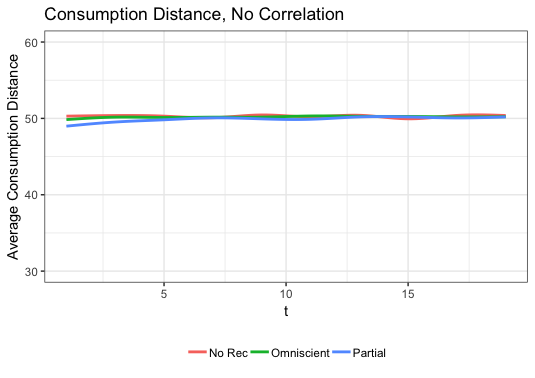
\includegraphics[scale=0.4]{figures/consumption_dist_N_200T_20no_correlation}
\caption{Consumption path with no correlation between utilities}
\label{fig:no_correlation_consumption_path}
\end{figure}

\begin{figure}
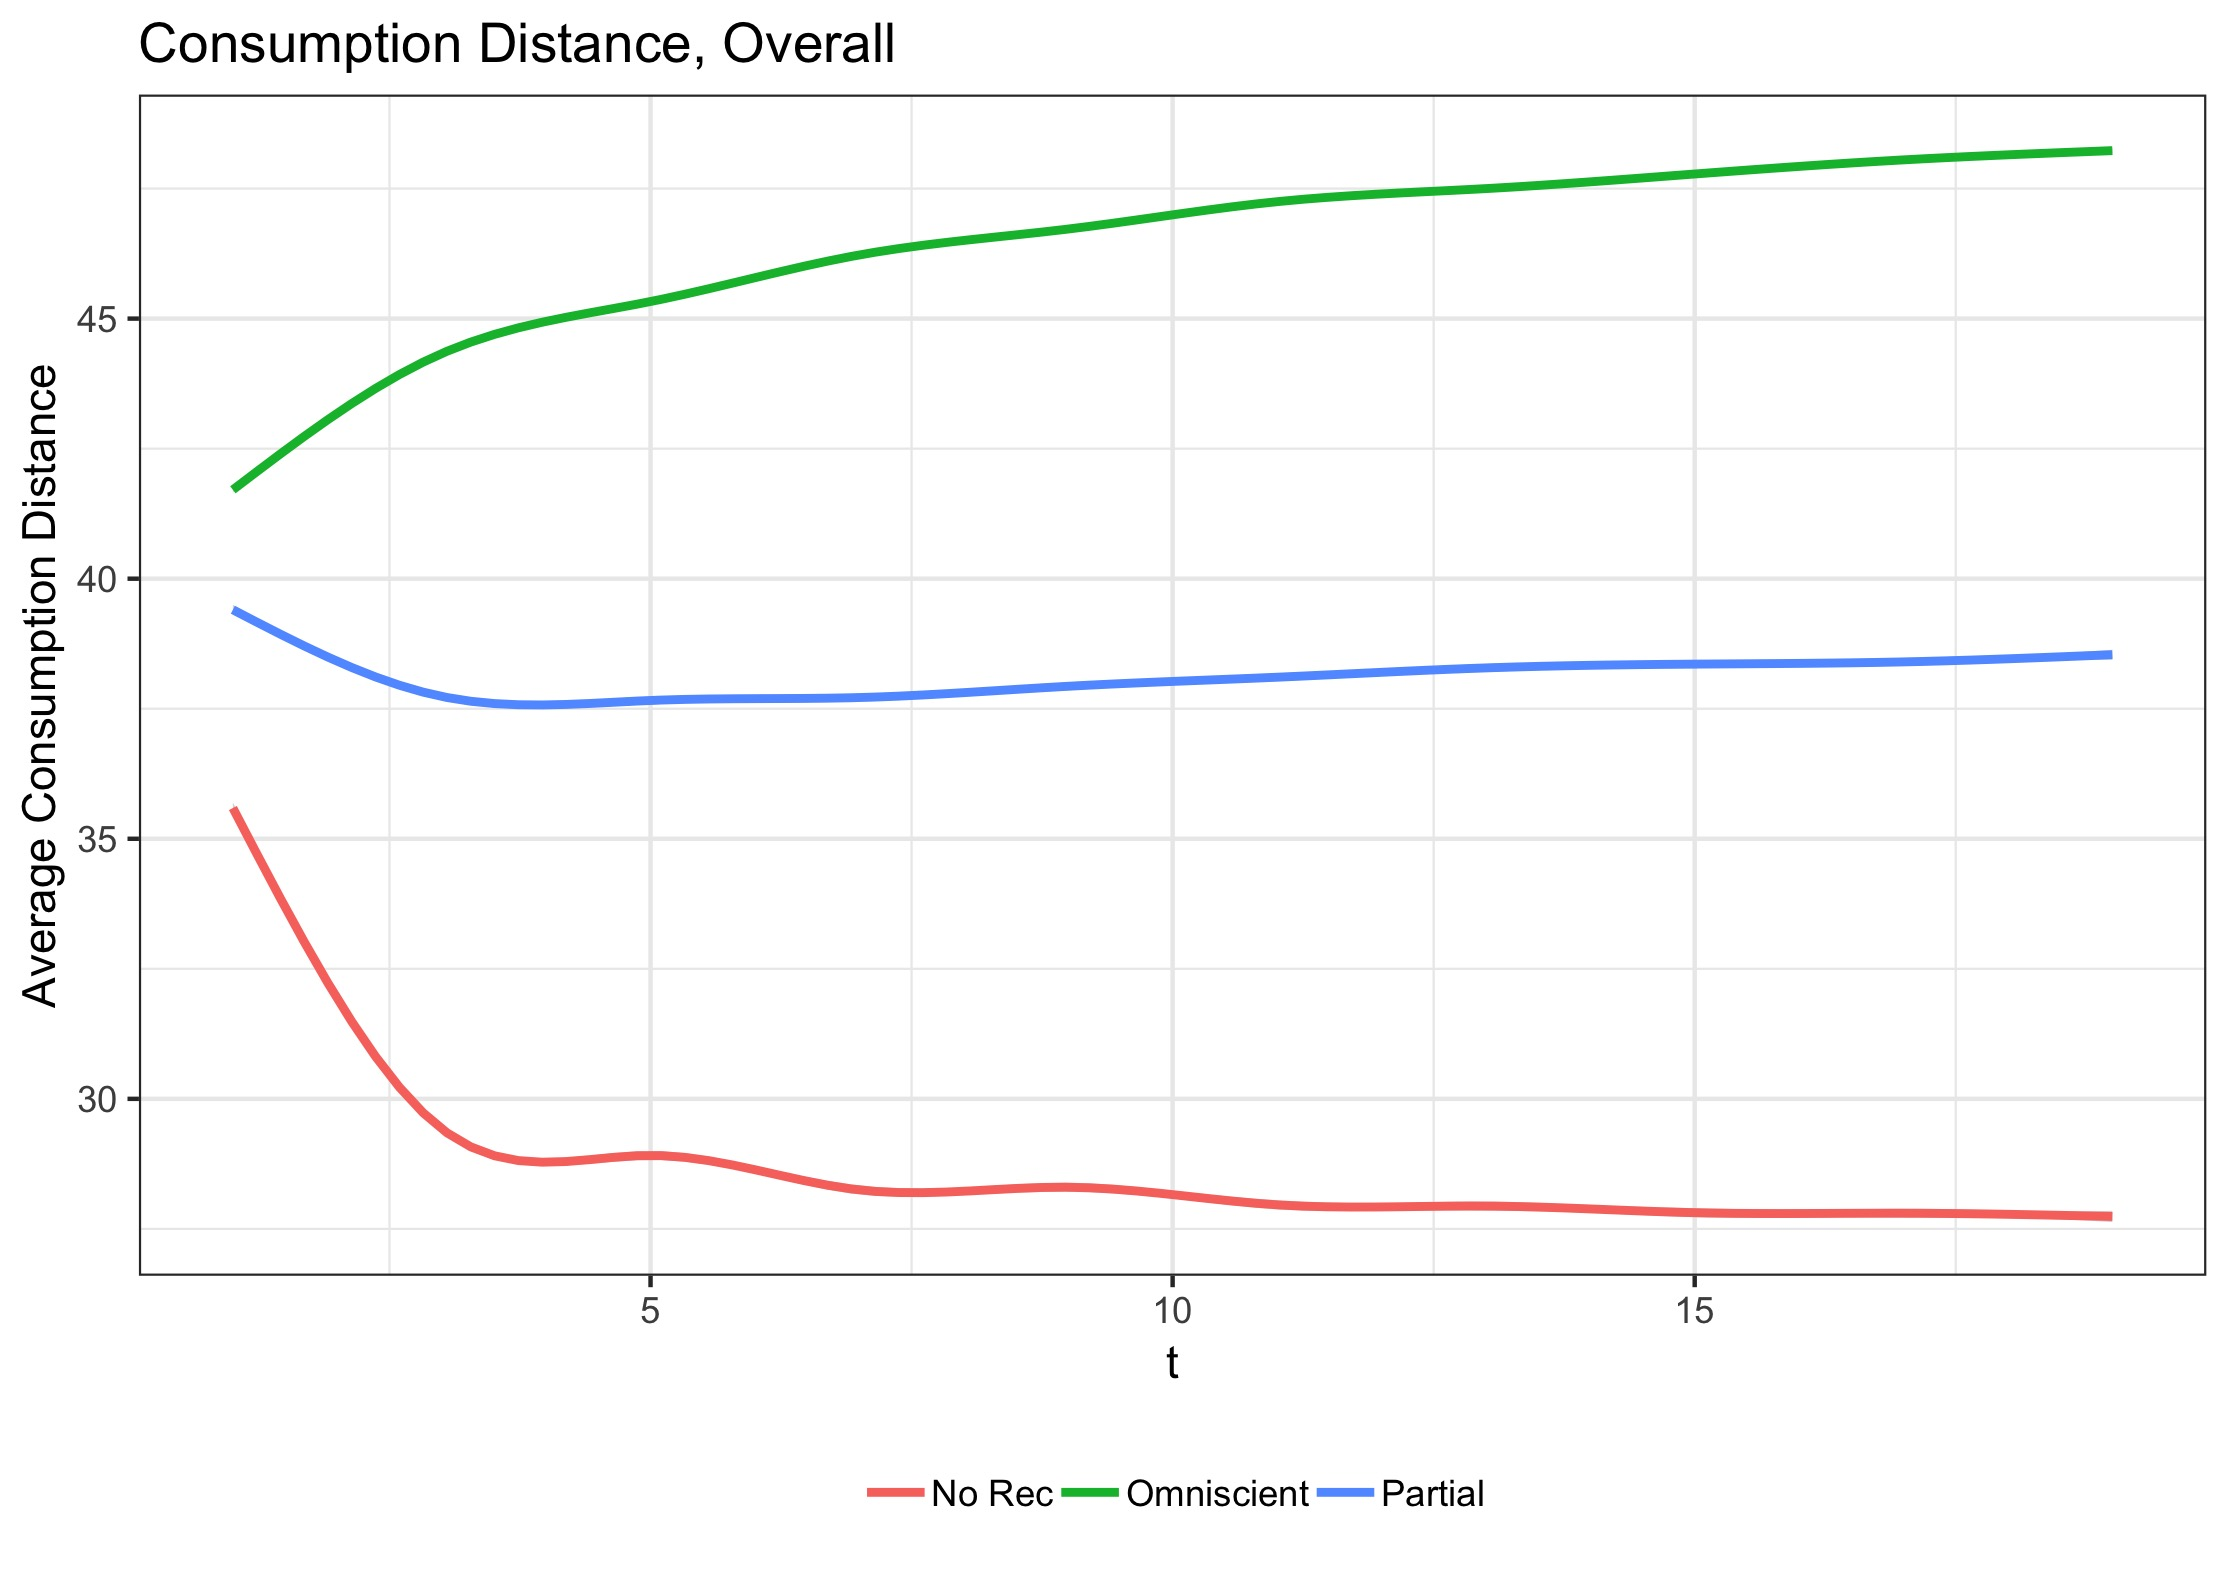
\includegraphics[scale=0.1]{figures/consumption_dist_N_200T_20_overall}
\caption{Consumption path between Recommendation Regimes}
\label{fig:consumption_path_between_regimes}
\end{figure}

We characterize ``filter bubble" effects in our model as the degree to which consumers engage in \textit{local consumption}. We define local consumption in terms of the average consumption distance between the items consumed by the representative consumer at time $t-1$ and $t$. We compare the average movement within the product space across different recommendation regimes and associate lower average distance with more local consumption.

\begin{finding}\label{finding_local_consumption}
The impact of recommendation on local consumption:
\begin{enumerate}
\item When $\rho = 0$, there is no difference in consumption distance between the three recommendation regimes.
\item When $\rho > 0$, no recommendation induces more local consumption than both partial and omniscient recommendation. This effect is amplified as $\rho$ increases as well as when consumers are more risk averse ($\gamma$ increases)
\end{enumerate}
\end{finding}

First, Figure \ref{fig:no_correlation_consumption_path} shows that, when $\rho = 0$, there is no difference in consumption distance between the three regimes. This is due to the fact that when $\rho = 0$, there is no reason that items that are close in the product space should have similar utilities and so the optimal consumption path does not depend on the similarity of the items. However this also means that consumers in the no recommendation regime do not learn anything about neighboring goods and so there is limited path-dependence in consumption.

Figure \ref{fig:consumption_path_between_regimes} shows that, when $\rho > 0$, both partial and no recommendation lead to increasingly local consumption compared to the benchmark omniscient case. Further, the average consumption path between periods is \textit{decreasing} for the no recommendation case whereas it is \textit{increasing} for the omniscient case. Partial recommendation decreases the degree of local consumption but not as much as the omniscient benchmark. Due to the correlation of utilities, the omniscient consumption path exploits this and leads to the consumption of more similar products than in the case when $\rho = 0$. However, since these spillovers also impact consumer learning in the no recommendation case, consumers \textit{over-exploit} this and increasingly consume products similar to good products that they have consumed before. This is further illustrated by Figure \ref{fig:local_consumption_across_rho} which shows how the consumption paths between omniscient and no recommendation vary as $\rho$ increases.

Finally, this effect is further amplified as the level of risk aversion, $\gamma$, increases. Figure \ref{fig:no_rec_risk_aversion} shows how drastically the degree of local consumption increases as $\gamma$ increases. This is due to the fact that the spillovers not only affect the mean expected belief about quality but also the degree of uncertainty. Local consumption therefore leads to consumers to have less uncertainty about certain areas of the product space and risk aversion may lead them to increasingly consume these products.

\begin{figure*}
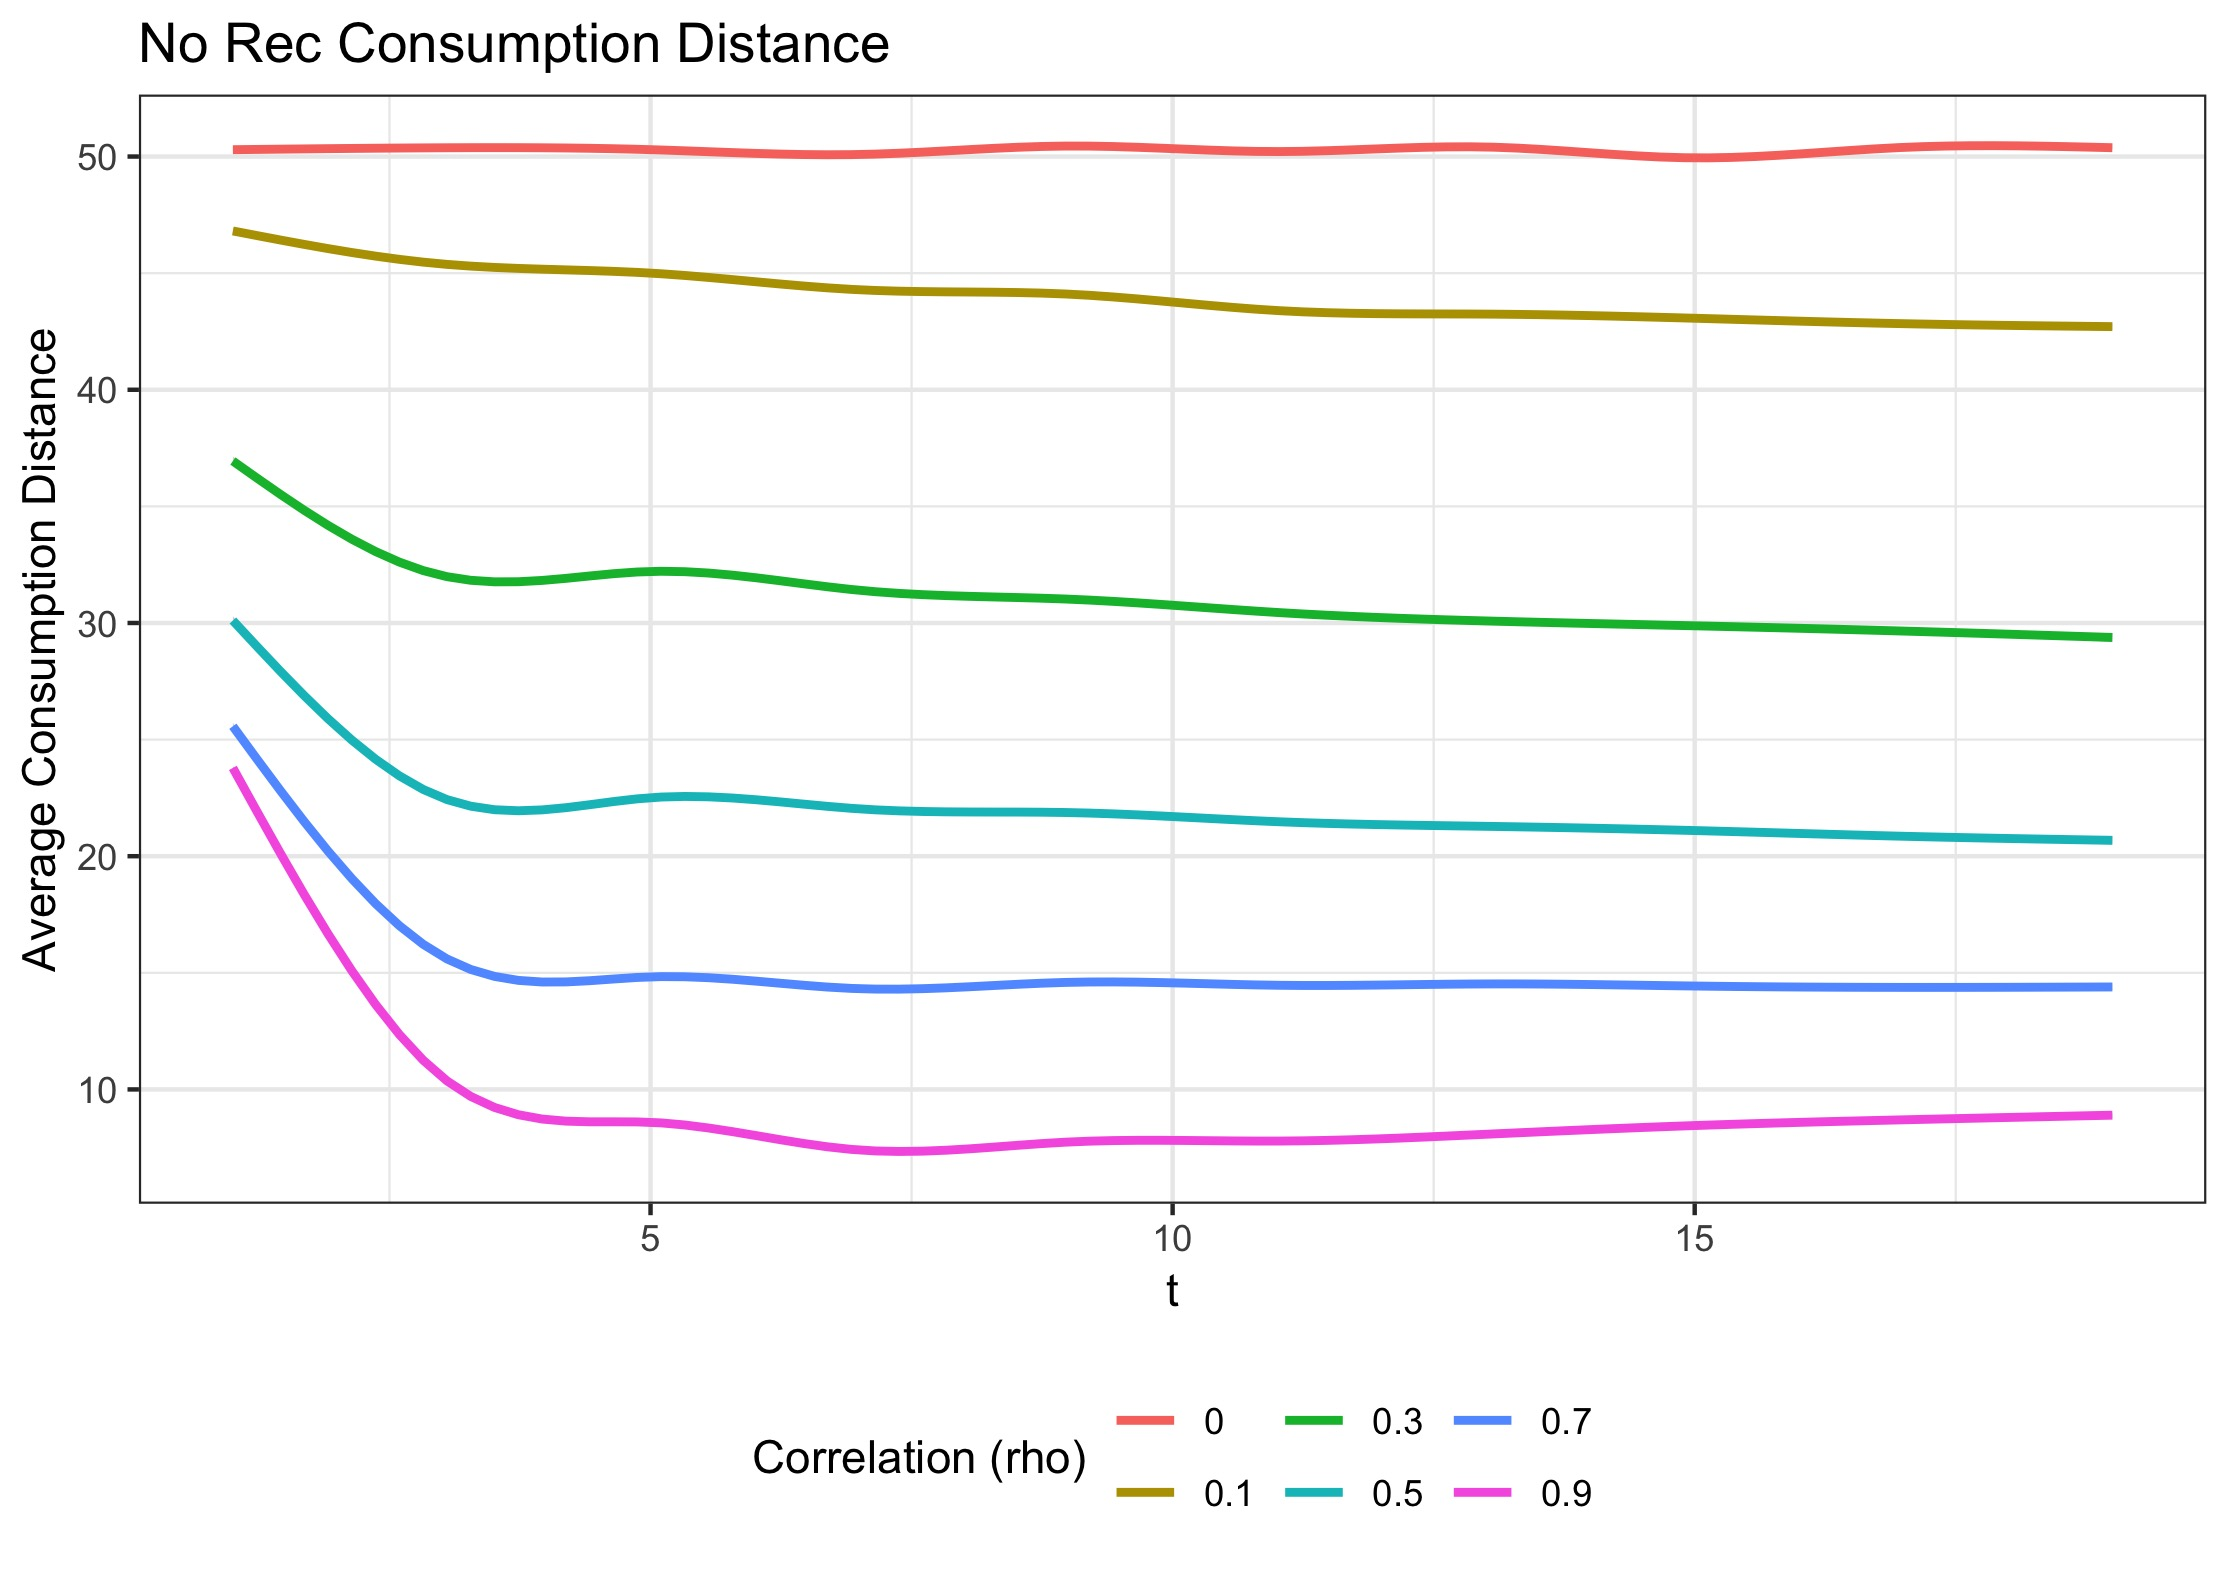
\includegraphics[scale=0.1]{figures/consumption_dist_N_200T_20_no_rec_rho}
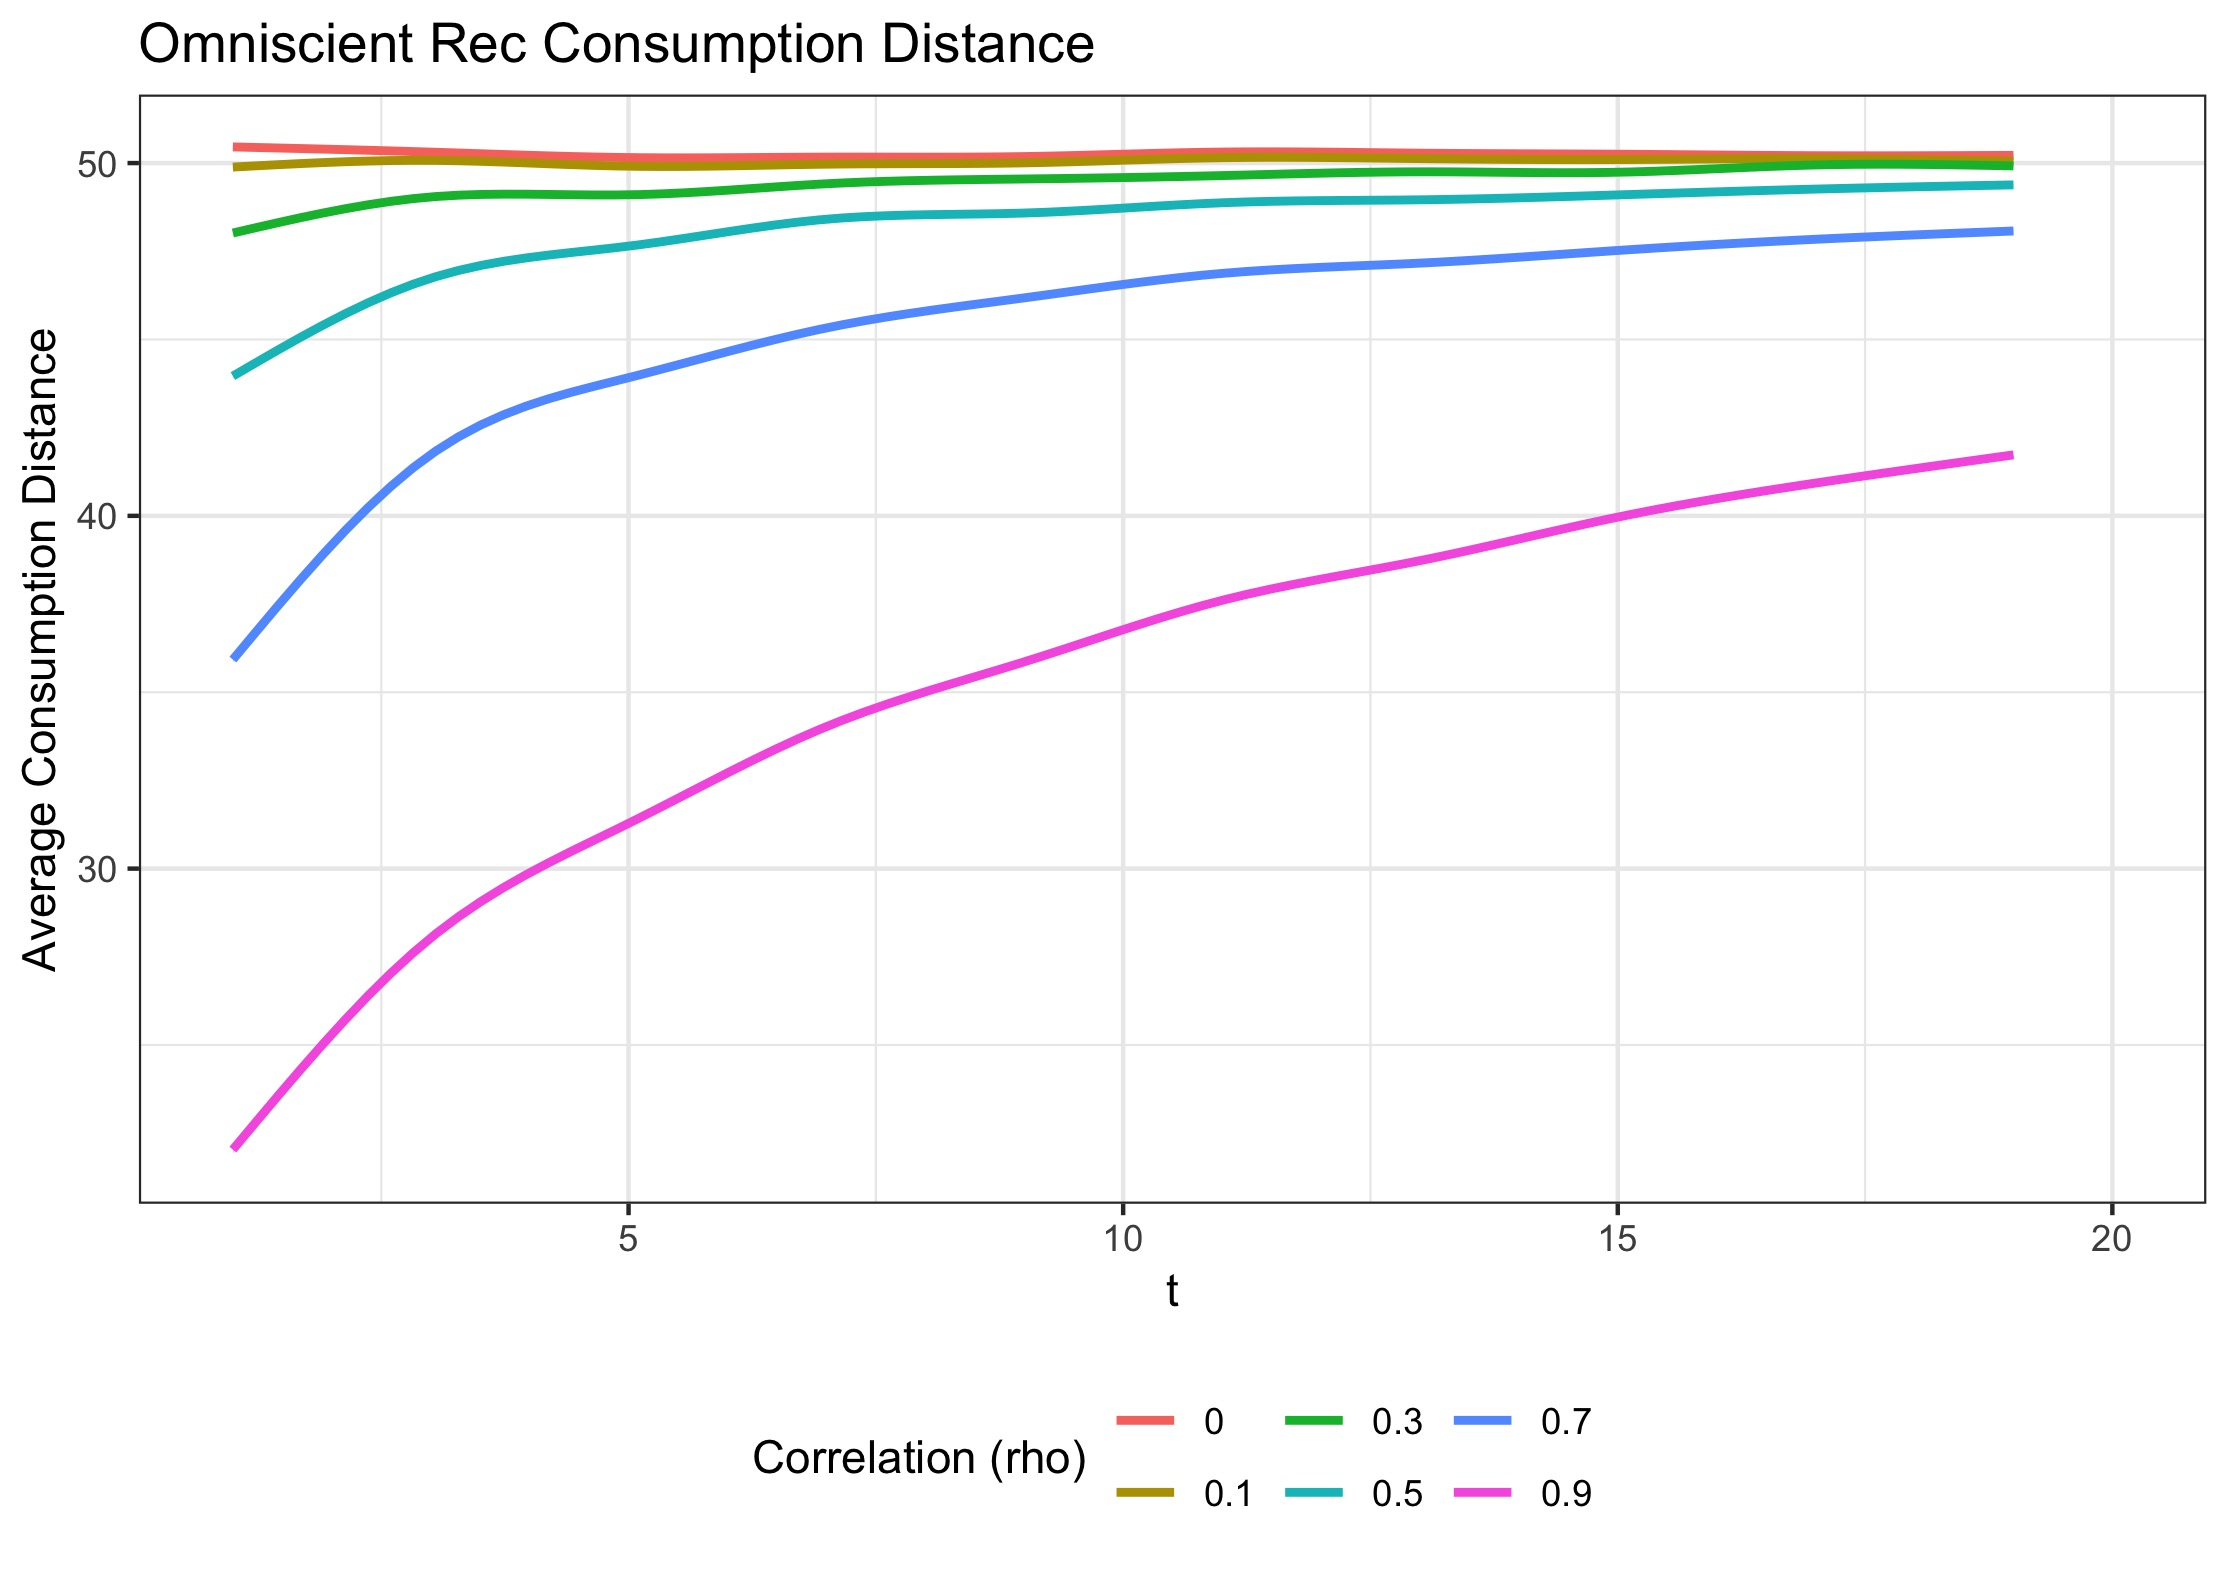
\includegraphics[scale=0.1]{figures/consumption_dist_N_200T_20_omni_rho}
\caption{Extent of Local Consumption for No Recommendation (Left) and Omniscient Recommendation (Right)}
\label{fig:local_consumption_across_rho}
\end{figure*}

\begin{figure}
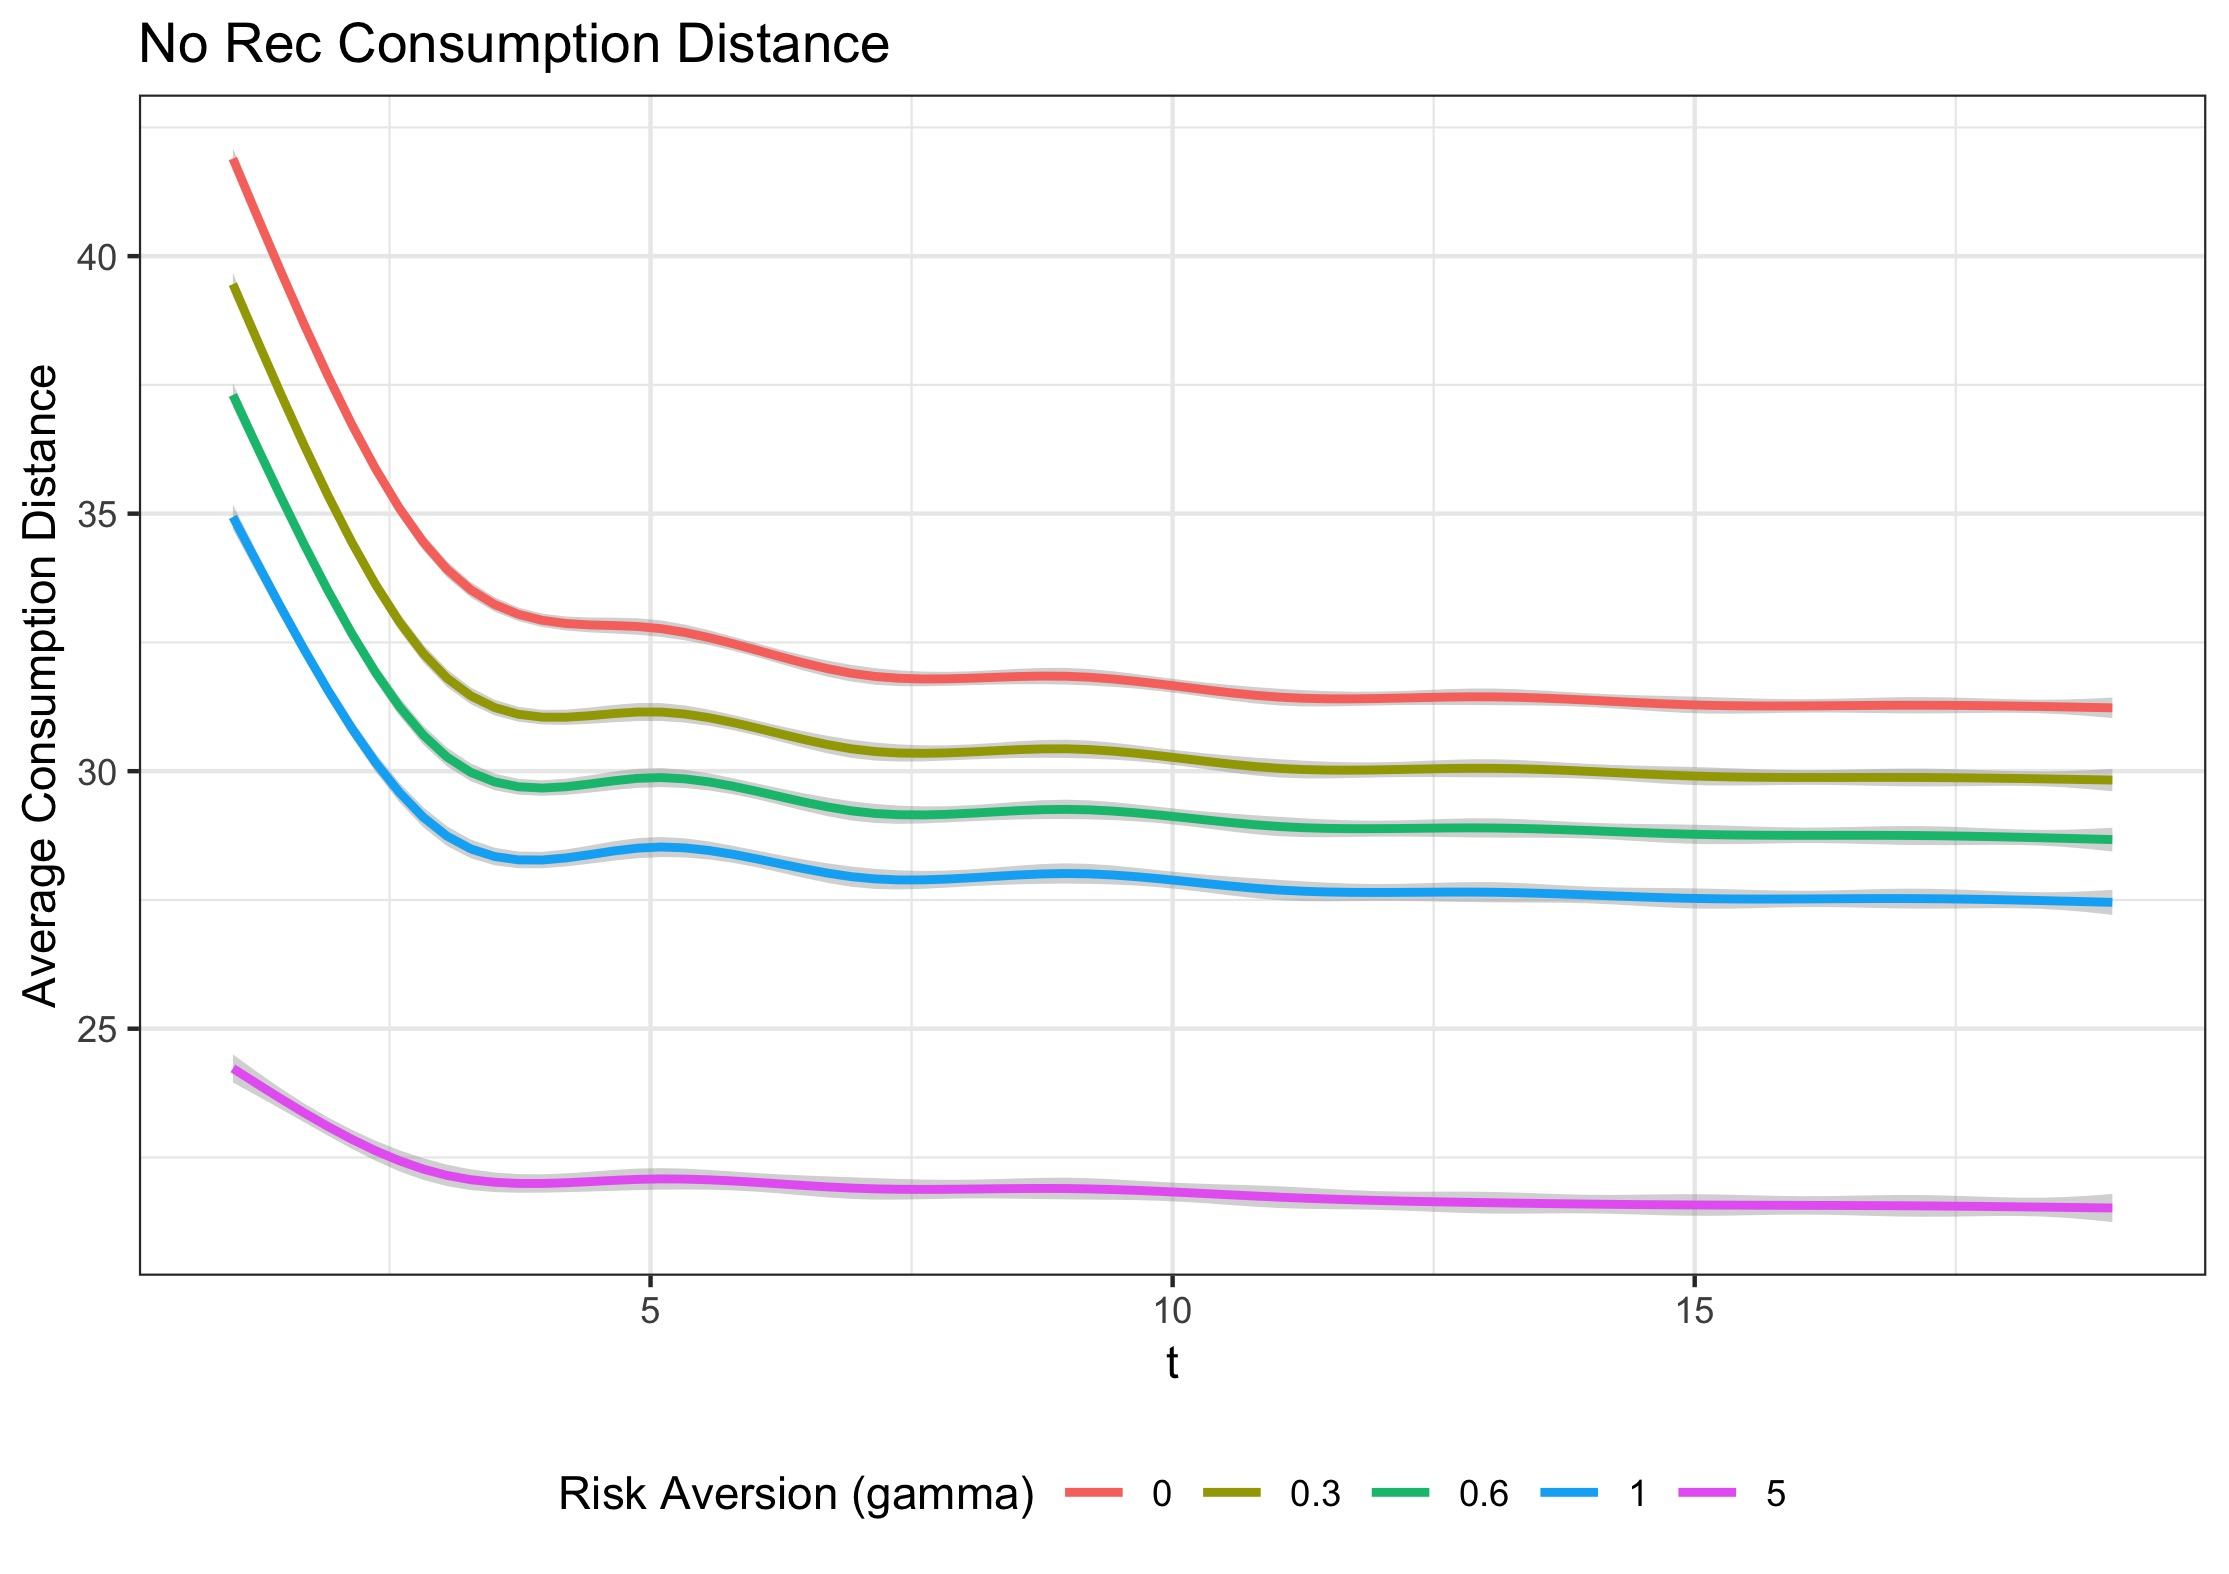
\includegraphics[scale=0.1]{figures/consumption_dist_N_200T_20_no_rec_alpha}
\caption{The Effect of Risk Aversion on Local Consumption}
\label{fig:no_rec_risk_aversion}
\end{figure}

\subsection{User Welfare and Product Diversity}

In this section we primarily focus on the impact of recommendation on the welfare on consumers as well as the overall diversity of the items that they consume.
Consumer's \textit{ex-post} welfare is the average of realized utilities, to control for the effect of $T$, and is defined as follows:
\begin{align*}
W_i=\frac{1}{T}\sum_{n \in C_i^T} u_{in}
\end{align*}
While in the previous section we looked at the distance between consecutive goods, we also define a diversity measure that is defined over the entire consumed set. We utilize a diversity metric common in the literature (e.g. \cite{ziegler2005improving}) which is the average normalized pairwise distance between the consumed products:
\begin{align*}
D_i =\frac{1}{N} \frac{1}{T (T-1)}\sum_{n,m \in C_i^T: n \ne m} d(n,m)
\end{align*}

\begin{finding}\label{finding_diversity}
The impact of recommendation on product diversity:
\begin{enumerate}
\item When $\rho = 0$, product diversity is the same across all three recommendation regimes.
\item When $\rho > 0$, product diversity decreases across all recommendation regimes but decreases the most in the no recommendation regime. This effect is amplified as $\rho$ increases as well as when consumers become more risk-averse.
\end{enumerate}
\end{finding}

As before, when there is no correlation between utilities product diversity is the same across different recommendation regimes. The over-exploitation of the learning spillovers when $\rho > 0$ leads to product diversity being lowest in the no recommendation regime. Figure \ref{fig:diversity_correlation} shows how diversity varies across recommendation regimes and the level of $\rho$ and Figure \ref{fig:risk_aversion_diversity} shows how diversity varies as risk aversion levels change. 

\begin{finding}
The welfare gap between no recommendation and partial recommendation as well as no recommendation and omniscient recommendation is decreasing in $\rho$.
\end{finding}
However, interestingly, the decrease in diversity is \textit{not} associated with a decline in welfare. In fact, welfare stays roughly the same in the omniscient case and slightly increases for the partial recommendation case. The welfare gap between the no recommendation case and the other two cases \textit{decreases} as the diversity gap increases.

\begin{finding}
Without recommendation, diversity and welfare are:
\begin{enumerate}
\item Negatively correlated when consumers have no risk-aversion
\item Uncorrelated when consumers have high levels of risk-aversion
\end{enumerate}
\end{finding}

Figure \ref{fig:diversity_welfare_ra} shows how diversity and welfare correlate for the no recommendation case. When there is no risk-aversion then there is a negative correlation between welfare and diversity. This is since, with no risk-aversion, in a given period a consumer will select the good that they currently believe has the highest expected value. High product diversity in this case can arise from a consumer who consumes a bad item and updates her beliefs about nearby items negatively. As a result, in the next period she will pick an item far away in the product space from the item that she consumed previously. If the item that she had consumed was ``good", then she is more likely to pick a nearby item. The learning spillovers therefore lead to high product diversity being negatively correlated with welfare.

\begin{figure}
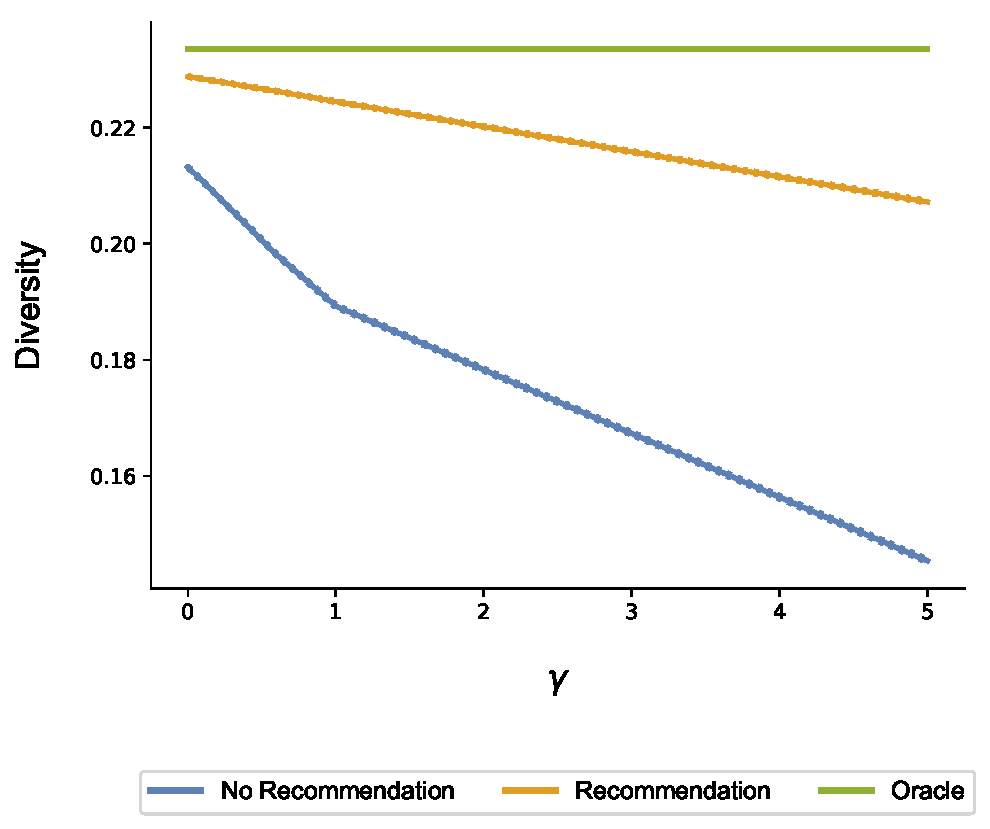
\includegraphics[scale=0.1]{figures/gamma_diversity_N_200_T_20}
\caption{Risk Aversion and Diversity}
\label{fig:risk_aversion_diversity}
\end{figure}

This only happens since $\gamma = 0$ leads to consumers only caring about the expected value of the good. However, as we saw in Findings \ref{finding_local_consumption} and \ref{finding_diversity}, increasing $\gamma$ can lead to lower diversity and increasingly local consumption due to the fact that the degree of uncertainty now impacts consumers' choices. This weakens the negative relationship between diversity and welfare since both negative and positive experiences with a good reduce uncertainty about surrounding goods. This leads to the inverted-U shape found in Figure \ref{fig:diversity_welfare_ra} when $\gamma$ is relatively large (e.g $\gamma = 5$).

\begin{figure*}
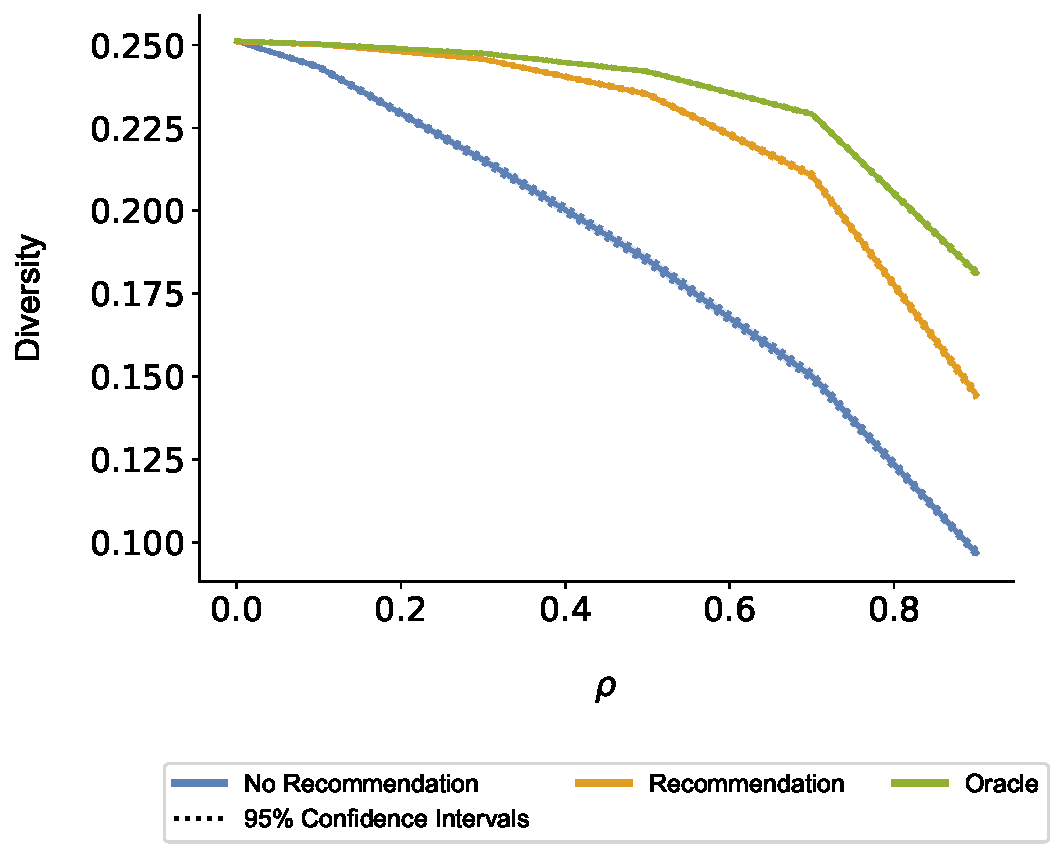
\includegraphics[scale=0.1]{figures/rho_diversity_N_200_T_20}
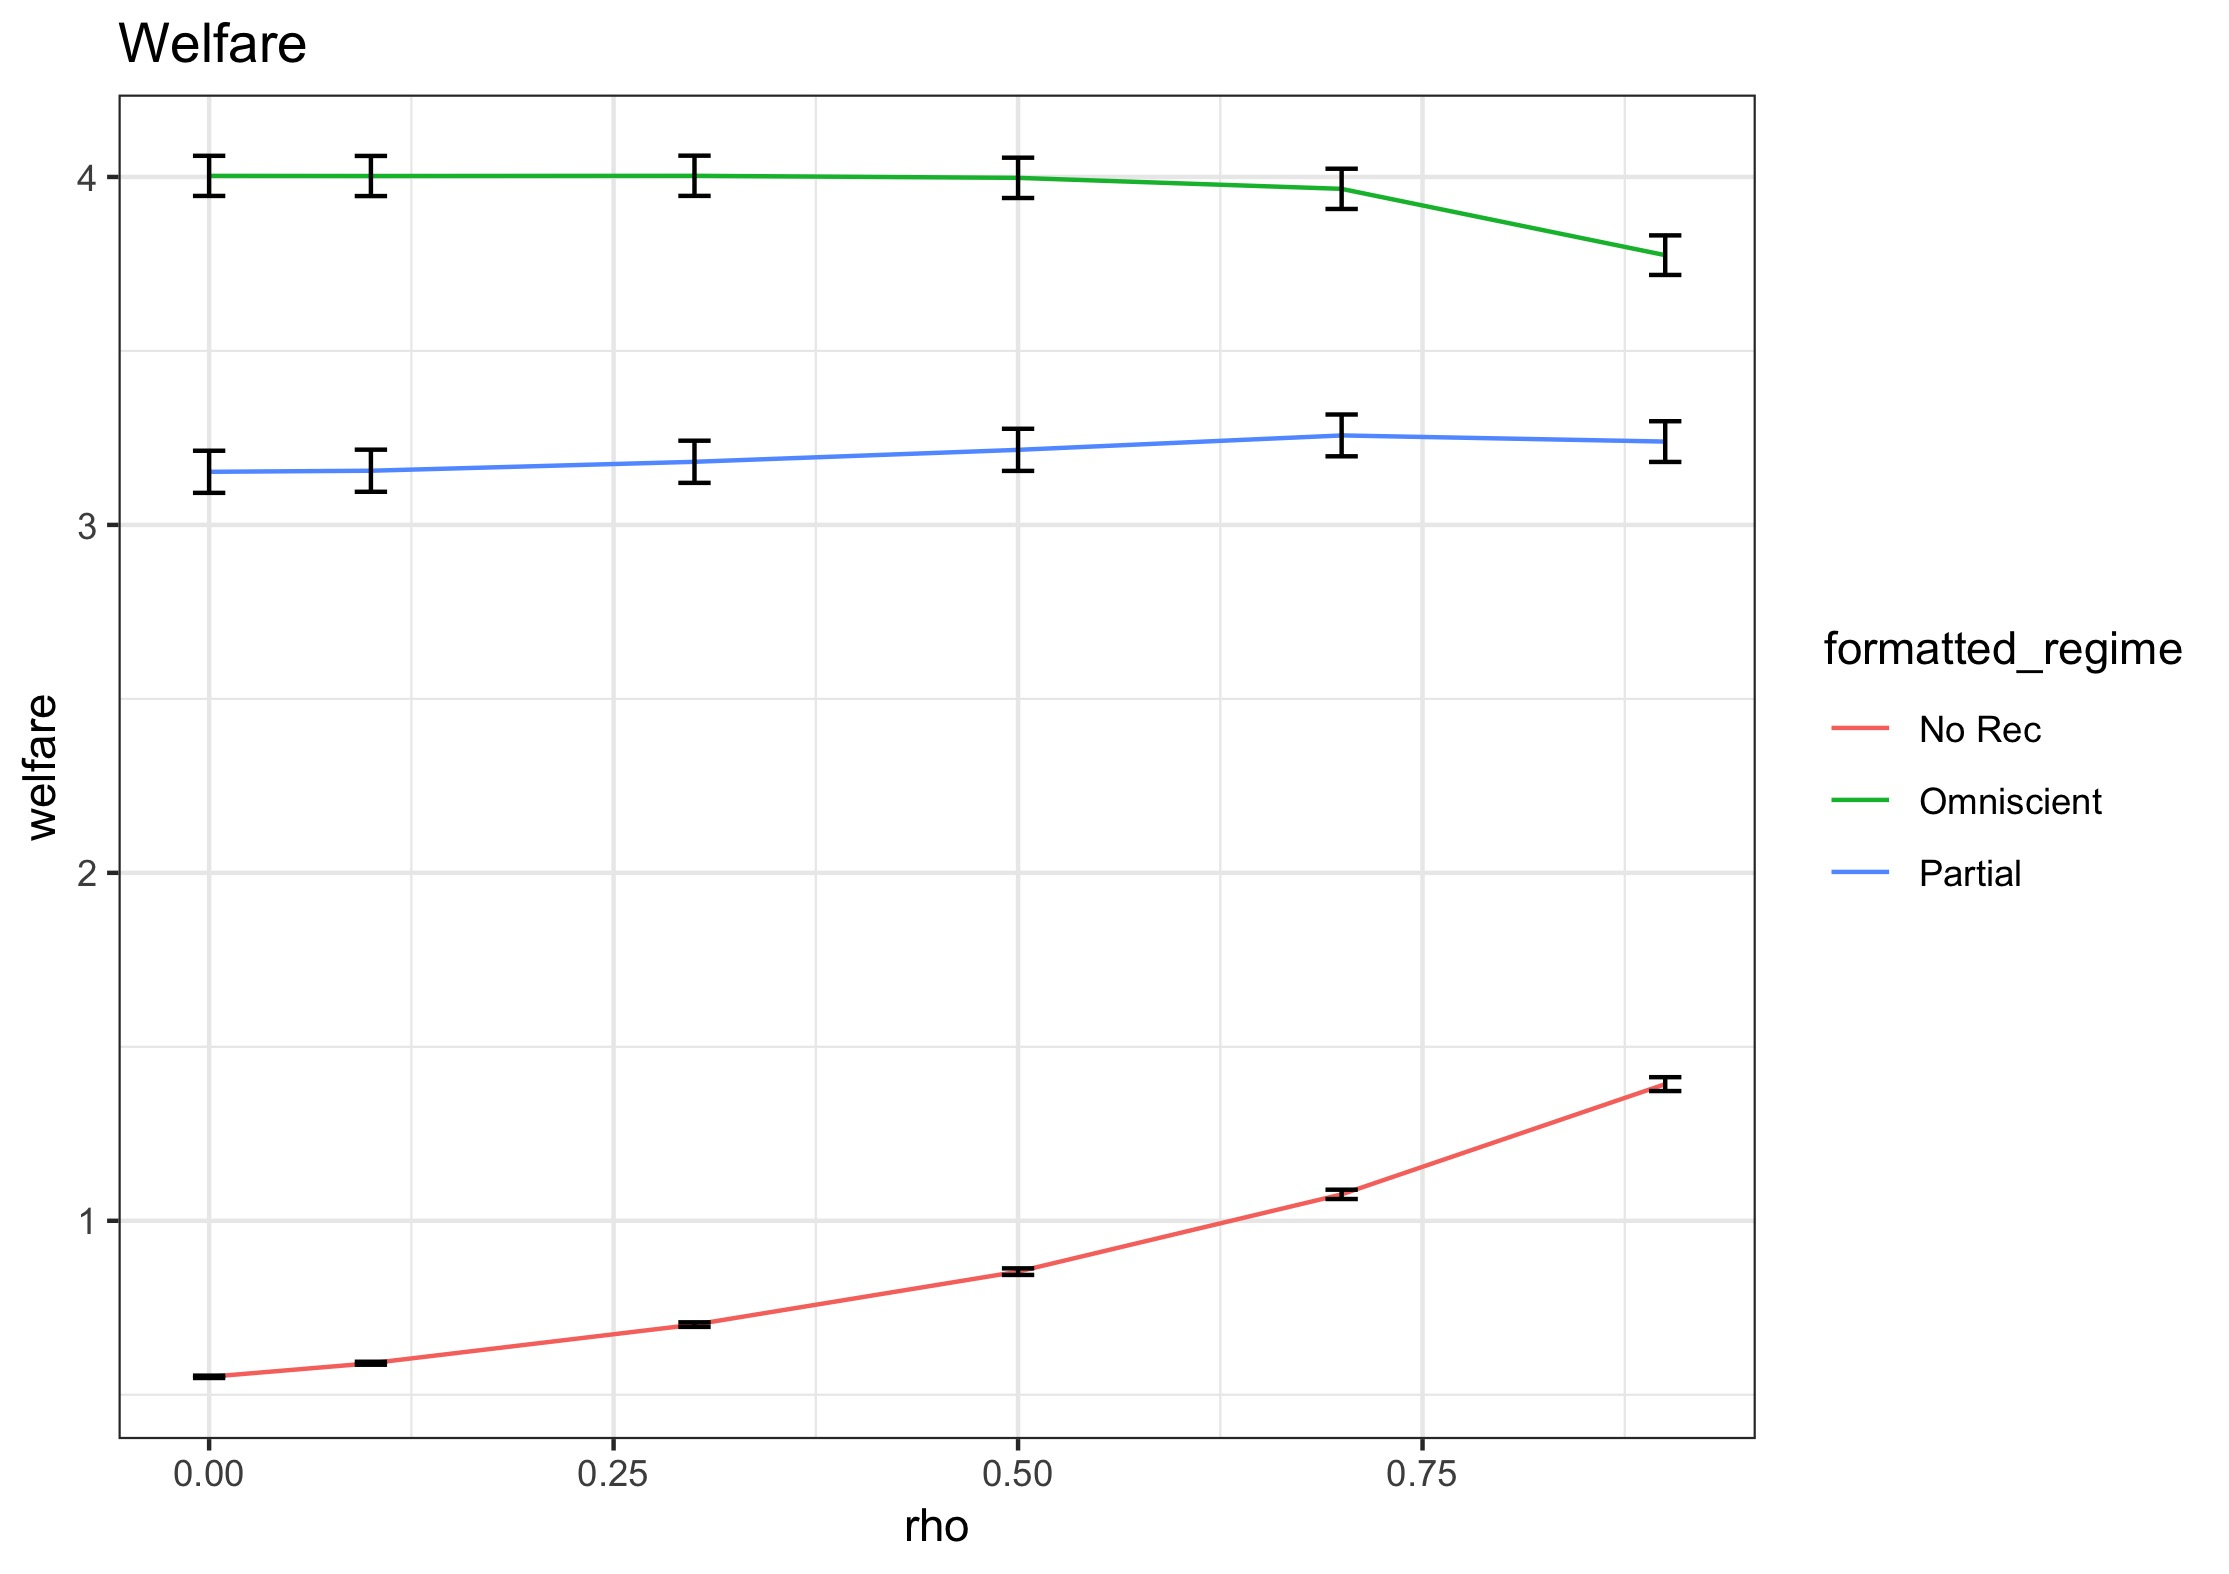
\includegraphics[scale=0.1]{figures/rho_welfare_N_200_T_20}
\caption{Welfare, Diversity, and Correlation}
\label{fig:diversity_correlation}
\end{figure*}

\begin{figure*}
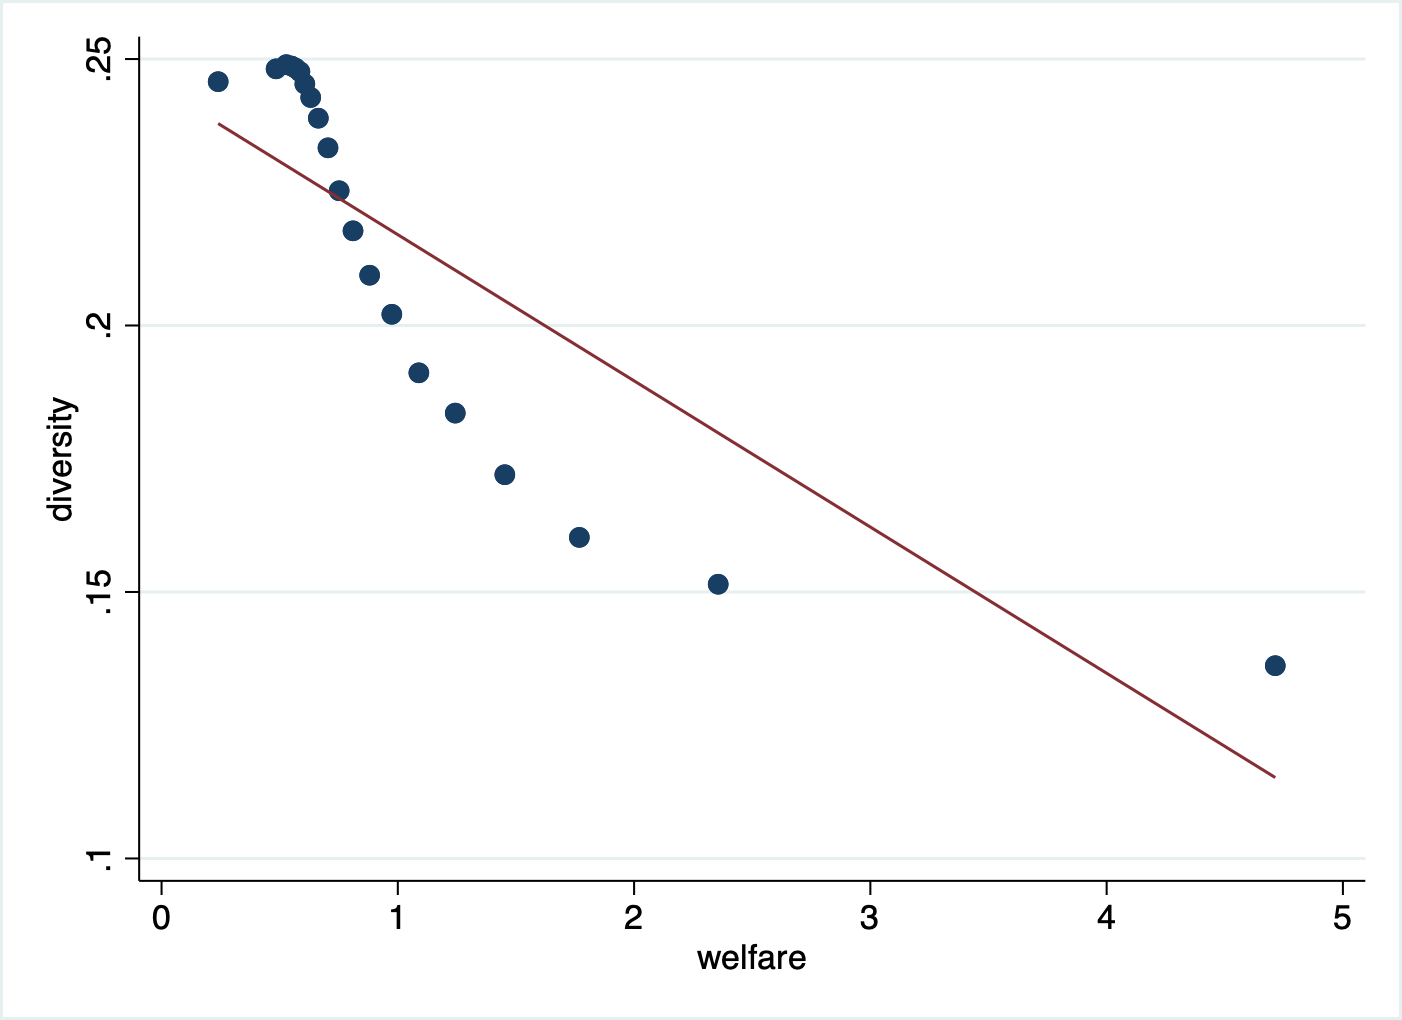
\includegraphics[scale=0.3]{figures/diversity_welfare_no_risk_aversion}
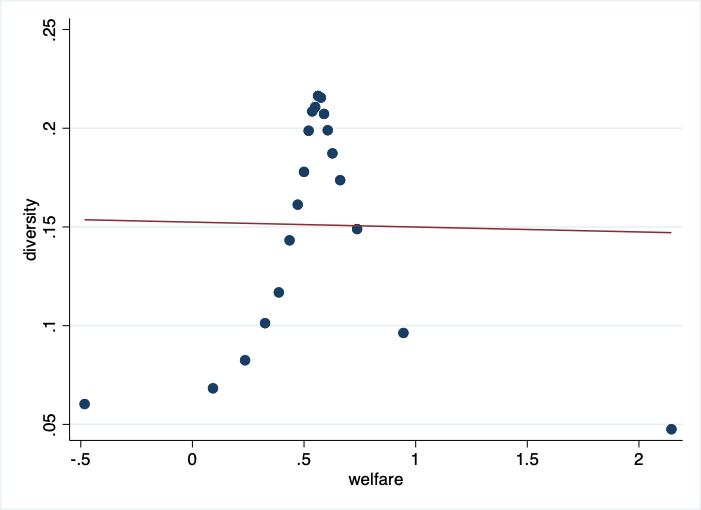
\includegraphics[scale=0.3]{figures/diversity_welfare_high_ra}
\caption{Diversity vs. Welfare, $\gamma = 0$ (Left), Diversity vs. Welfare, $\gamma = 5$ (Right)}
\label{fig:diversity_welfare_ra}
\end{figure*}

\subsection{User Homogenization}

In this section we focus on across user comparisons and investigate how the consumed set of items across consumers varies across different recommendation regimes and parameter values. In particular we look at the degree of \textit{homogenization} between consumers. Similar to \cite{chaney2018algorithmic} we use the Jaccard index between the consumption sets of consumers to measure homogeneity:
\begin{align*}
H:=\frac{1}{|I|(|I|-1)}\sum_{i,j \in I: i \ne j}d_J(C_i^T,C_j^T)
\end{align*}
where $d_J$ denotes the Jaccard index and $H \in [0,1]$.
\begin{finding}
Homogeneity is:
\begin{enumerate}
\item Highest under partial recommendation and lowest under no recommendation
\item Increasing in $\beta$, or the weight of the common-value component
\item Decreasing in $\rho$ for partial recommendation, but weakly increasing in $\rho$ for no recommendation
\end{enumerate}
\end{finding}

Figure \ref{fig:beta_homo} shows that as the weight of the common-value component, $\beta$, increases consumers consume increasingly similar sets of items. The homogenization effect is strongest under partial recommendation since the revelation of the common-value component induces consumers to consume products in similar areas of the product space. However, as $\beta$ increases, some amount of homogenization is optimal as can be seen from the omniscient recommendation case. In the no recommendation case since consumers do not know the common-value component they engage in local consumption in different areas of the product space which leads to less than optimal homogeneity.

Figure \ref{fig:cor_homo} shows that the degree of homogeneity in the partial recommendation case however is \textit{decreasing} as $\rho$ increases. As was discussed in Findings \ref{finding_local_consumption} and \ref{finding_diversity}, the degree of local consumption increases with $\rho$. Even though the revelation of the common-value component induces them to search in similar parts of the product space, their idiosyncratic components induce them to consume products in a more localized area of the product space as $\rho$ increases which leads to a decline in homogeneity.

\begin{figure}
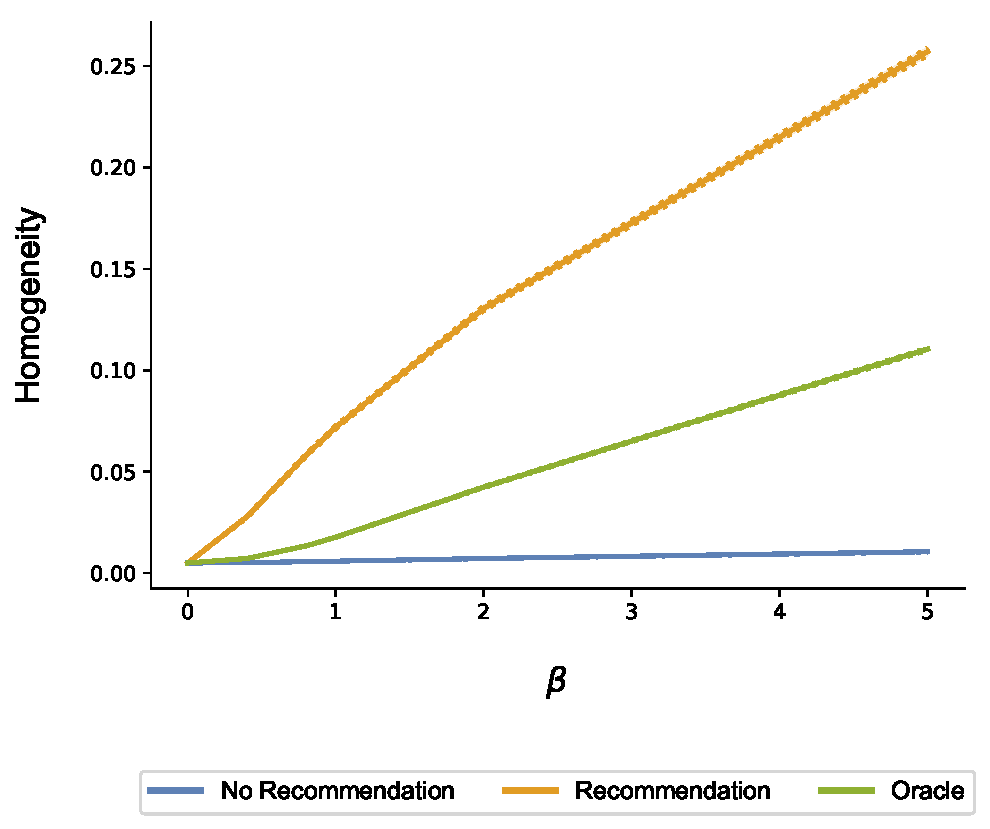
\includegraphics[scale=0.1]{figures/beta_homogeneity_N_200_T_20}
\caption{Strength of Recommendation and Homogeneity}
\label{fig:beta_homo}
\end{figure}

\begin{figure}
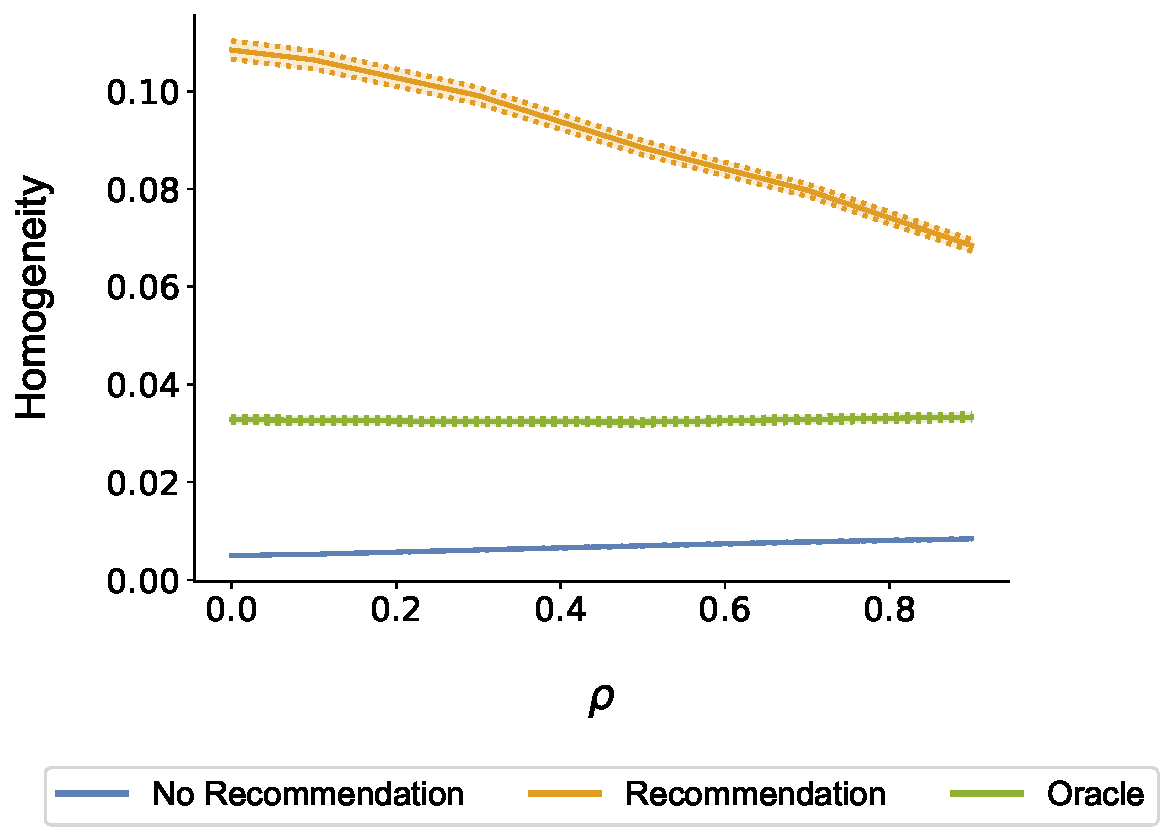
\includegraphics[scale=0.1]{figures/rho_homogeneity_N_200_T_20}
\caption{Correlation and Homogeneity}
\label{fig:cor_homo}
\end{figure}



\subsection{Effectiveness of Recommendation}


\section{The Value of the Ex-Ante View}

In this section we illustrate the differences between the ex-post and ex-ante view and show how it is useful for thinking about the design of RS. Our first point is trivial to state - since users do not know the true consumption values of the items, without any further information they may make \textit{ex-post} sub-optimal consumption decisions, but \textit{ex-ante} optimal given the information available to them at the moment of choice. Consider the following stylized example. The choice set of the individual is $\Omega= \{x_1, x_2, x_3 \}$ and the ex-post utility values are given by
$u(x_1) = 1$, $u(x_2) = 2$, $u(x_3) = 3$. 
\par
However, when users are making decisions they have unobservable \textit{beliefs} about the ex-post utility value of the items and make decisions given these beliefs. As users obtain more information, their beliefs converge to the ex-post utility values but, generally, users do not have enough information and so have beliefs over the space of possible ex-post utility values. In this example we suppose these beliefs are simple so that users view each good as simple lotteries: for $n=1,2,3$, $u(x_n) = n + \varepsilon_n$, $\varepsilon_1 \sim \mathcal N (2, 1)$, $\varepsilon_2 \sim \mathcal N (0, 1)$, $\varepsilon_3 \sim \mathcal N (-5, 2)$.
\par
After uncertainty is unresolved, the user would consume $x_3$, but an expected utility maximizing consumer (without further information) would choose $x_1$.\footnote{We ignore an important component of decision-making under uncertainty, risk attitudes, by focusing on risk-neutral consumers. A \textit{risk-averse} user may choose to consume a good with lower expected \textit{ex-post} payoff but lower ex-ante variance compared to another good. While risk-aversion is important for decision-making under uncertainty, especially in the context of RS, it is not our main focus here.}
\par
This observation, while seemingly trivial, has important implications. The fact that the user would choose $C$ over $A$ reveals that $C$ prefers $A$ given her current beliefs\footnote{This is a statement of \textit{revealed preference} which has been studied heavily in economic decision theory (see e.g. \cite[]{mas1995microeconomic}).} and allows the system designer to get some information about a user's beliefs. Why are user beliefs important objects for designers of RS to understand and utilize?
\par
Beliefs are useful for understanding how users interact and get value from RS. In particular, users use RS to get \textit{information} about the set of items and update their beliefs about the value of the items. For instance, in the example, a RS could recommend to a user $x_3$ over $x_2$ and $x_1$ and that user will use this to update her beliefs about $x_3$. It is an empirical question that we leave for future work precisely how and to what extent users update their beliefs from recommendation and what factors of RS deisgn influence this.\footnote{There has been some work in this direction in understanding when recommendations are persuasive \cite{cremonesi2012investigating, gretzel2006persuasion} as well as the effect of their delivery on effectiveness \cite{murphy2014recommendation}.}
\par
Better understanding user beliefs is important for improving the performance of RS that optimize for metrics that move away from accuracy such as serendipity \cite{kotkov2016survey}. Serendipity-based RS attempt to provide recommendations that ``have the quality of being both unexpected and useful" \cite{maksai2015predicting} but it is hard to know what items are both unexpected and useful \cite{kotkov2016survey}. Understanding \textit{why} a user has not consumed a good depends on the beliefs that the user has and this is important for designing serendipitious recommendations. For instance, in the example, the user does not consume $x_3$ because she expects the good to turn out worse than the other two. However, if given more information, she would prefer to consume it over $x_1$ and $x_2$. Moreover, when the user can use her known valuation of an item to make inferences on how good another item is, consumption is path-dependent, as beliefs guide consumption and consumption affects beliefs about other goods. For instance, learning the value of $x_1$ says something about how good $x_2$ is. %When considering risk-averse individuals, when the user has alternatives with a known value,The consumer may have also consumed Another reason why the user may not . The user may have an alternative with a known value -- say going for a walk around the neighborhood -- which she could always prefer to watching a given movie that has uncertain value but that the consumer thinks is always lower than the value of the walk.\footnote{An additional reason this could be useful is if one considers a risk-averse individual, then it may be that a user has not consumed an item because she has a high perceived variance for the item's quality.}
As a result, understanding the beliefs of users helps us understand why users have not consumed certain items and, in particular, which items a user may find useful given more information about it. This poses an important problem: designing systems that elicit not only ex-post valuations but also ex-ante beliefs about valuations, as only by knowing these can RS be effective in steering users' choices. In particular, choice has to be perceived as guided by ex-ante utility, whereas ratings by the ex-post realized utility.
\par
Understanding the choices that individuals will make in addition to what they will end up liking are complementary problems but require different viewpoints. \cite{jiang2014choice, saavedra2016choice} argue that choice-based approaches alone can help in designing better RS, though they argue for these approaches because they do a better job at providing more accurate recommendations. We argue that the two problems should be considered separately -- though they may interact in interesting and useful ways.\footnote{In particular, some results in \cite{jiang2014choice, saavedra2016choice} may be driven by the fact that user choice embeds ratings information that may not have been observed by the recommender but is observed by the user. Ratings, reviews, friends, there are many sources of information affecting a person's beliefs and choices that are unobservable by RS. Other consumption choices, e.g. movies seen in the cinema, change beliefs about for instance how good a director is, which affect beliefs about other movies and guide choices on a streaming platform that is unable to observe these data.} 
\par
RS are designed to give users \textit{information} that is useful to help them make decisions. On the one hand, predicting a user's ex-post preferences is useful to know what items the user would like to consume. On the other hand, predicting what items a user will actually consume (without recommendation) can help reason about what information may actually be useful to give her. Furthermore, in designing RS to avoid filter bubble and homogenization effects, having accurate choice predictions allows mitigating such adverse effects to become a first-order component of design. In particular, by predicting both choice and ratings, RS can provide information to users that leads them to useful items but prevents them from falling into a filter bubble. 
\par
Solving this choice prediction problem requires data on the choices that individuals make and the sets that they choose them from in addition to the traditional ratings or behavioral data that is collected. In the example given previously the fact that the consumer chooses $x_1$ from the set $\{x_1, x_2, x_3 \}$ would be the data that is useful for the choice prediction problem, as would the consumer's ex-ante beliefs about her valuation of the goods.


\section{Conclusion}

We have argued that incorporating user choice under uncertainty should be a first-order component of RS design. By collecting appropriate data about user choices and user beliefs, RS can be built to better understand what choices users are likely to make and thus what information would be useful to give them as opposed to simply predicting what items a user will like. This approach can not only aid in designing more useful RS, but can also be utilized to better understand and prevent recently documented adverse effects of RS such as filter bubbles and homogenization.

\bibliographystyle{plain}
\bibliography{refs}
\end{document}
